%%%%%%%%%%%%%%%%%%%%%%%%%%%%%%%%%%%%%%%%%%%%%%%%%%%%%%%%%%%%%%%%%%%%%%%%%%%%%%%%%%%%%%%%%
% LICENSE NOTICE (CC BY 4.0)
%
% Author/Creator: Alexander Menzel
% Copyright: 2025 MitaTherm
%
% This work is licensed under the Creative Commons Attribution 4.0 International License.
% License Text (URI): https://creativecommons.org/licenses/by/4.0/
%%%%%%%%%%%%%%%%%%%%%%%%%%%%%%%%%%%%%%%%%%%%%%%%%%%%%%%%%%%%%%%%%%%%%%%%%%%%%%%%%%%%%%%%%

\chapter{Theoretical fundamentals and state of the art}
\label{chap:Theoretical fundamentals and state of the art}
%
A radiator thermostat is a device, which is mounted on a radiator valve to control the flow of hot water through the radiator. By this means it regulates the temperature of a room.

As described in \cite{ELVjournal.2012} and shown in figure \ref{fig:rt-photo}, a digital radiator thermostat typically consists of the following components:

\begin{itemize}
	\item \acs{pcb} with \ac{ui} including buttons, rotary encoder, display, motor driver, and other components
	\item \ac{dc}-motor
	\item Gear box with planetary gears
	\item Valve connector
\end{itemize}

Most digital thermostats are \ac{mcu}-based and battery powered. Smart thermostats often include additional features such as \ac{wlan} or \ac{ble} connectivity and mobile app integration. 

Descriptions of common thermostats such as eQ-3 MAX! from \cite{ELVjournal.2012} and smart eQ-3 eqiva Bluetooth from \cite{eQ3AG.05.2018} can be used as a reference for functional scope of the software to develop. For example they implement following functions:

\begin{itemize}
	\item Mode selection (Auto, Manual, Boost, Vacation)
	\item Manual temperature adjustment
	\item Weekly schedule programming
	\item Open-window function
\end{itemize}

\begin{figure}[htbp]
	\centering
	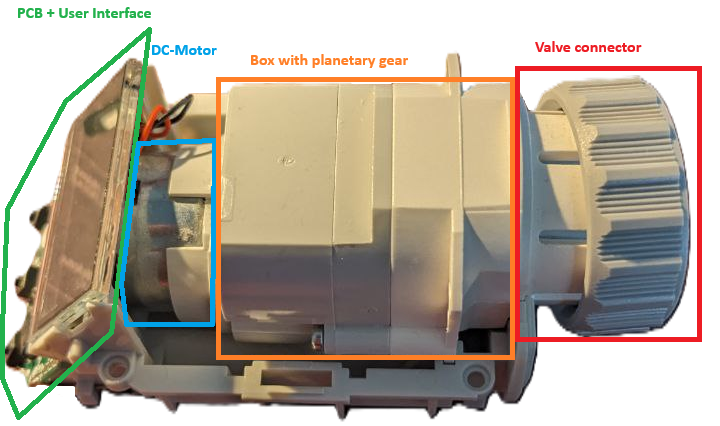
\includegraphics[width=0.9\linewidth]{./content/images/photo_2025-10-15_07-17-45_mod.png}
	\caption{Photo of a partially disassembled radiator thermostat eQ-3 eqiva (version without Bluetooth).}
	\label{fig:rt-photo}
\end{figure}